\section{Fermionic space to spin space transformations}\label{sec:Encoding}

The core part of the VQE algorithm is the measurement of the expectation value of the Hamiltonian operator (Eq. \ref{eq:molecularhamiltonianladder}) with respect to a parameterized ansatz wavefunction.  As mentioned in the previous section, in the NISQ era, with a limited number of qubits available, second quantization formalism has been favored over first quantization for quantum simulation. The fermionic creation and annihilation operators in second quantization formalism obey the anti-commutation algebra (Eq. \ref{eq:anticommutation}).

Qubits in comparison are spin-$1/2$ objects, and as such, the only operators that can, in general, be directly measured on QPUs are spin-operators (or the Pauli operators, $X$, $Y$, and $Z$) which obey a different algebra specified by their Lie bracket. This means that before starting the VQE loop, one must transform the Hamiltonian in second quantization into a linear combination of Pauli strings (tensor product of Pauli operators on multiple qubits). 

As discussed in Sec. \ref{sec:second_quantization} however, operators in second quantization must enforce the antisymmetry of the wavefunction and as such must obey anti-commutation rules as detailed in Eq.~(\ref{eq:anticommutation}). Pauli operators do not naturally obey these relationships and therefore specific cares must be brought to the mapping of fermionic operators to spin operators in the case of second quantization. 

All transformations can be formalized as 
\begin{equation}
    \mathcal{T}: \mathcal{F}_n \rightarrow (\mathbb{C}^2)^{\otimes N},
\end{equation}
where a transformation $\mathcal{T}$ maps the space of operators acting on Fock states of $n$ spin orbitals, $\mathcal{F}_n$, to the Hilbert space $(\mathbb{C}^2)^{\otimes N}$ of operators acting on spin states of $N$ qubits. The most important feature of the transformation is that it must maintain the anti-commutation of fermionic operators. Conveniently, Jordan and Wigner \cite{Jordan1928} showed long before Quantum Computers were even conceptualized that an isomorphism exists between fermionic space and qubit space, maintaining the algebraic structure. 

It is important to note that the mappings described in this section not only affect the operators measured when computing the expectation value of the Hamiltonian, but also the construction of an ansatz that is initially defined in fermionic terms (for instance the Unitary Coupled Cluster ans{\"{a}}tze, see Sec. \ref{sec:UCCA}). These ans{\"{a}}tze must be transformed into a series of Pauli operators exponentials which can be implemented as quantum gates.

In this section, we present a number of such transformations. There are three main characteristics relevant to deciding on a specific encoding, although it is worth noting that these are not necessarily independent from each other:
\begin{itemize}
    \item \textbf{Number of qubits:} The number of qubits required to represent the electronic wavefunction. In general, the number of qubits is directly proportional to the number of spin-orbitals or sites considered. However, several techniques have been developed to concentrate the information held in the wavefunction to as few qubits as possible \cite{Moll2016, bravyi_tapering_2017, Steudtner2018, Setia2020, Kirby2021_CSVQE}. These methods generally rely on symmetries of the Hamiltonian and are presented in the last part of this section. 
    \item \textbf{Pauli weight:} The maximum number of qubits on which each Pauli string produced act, i.e. the maximum number of non-identity operators in any Pauli string produced by the mapping. This is, in general, referred to as Pauli weight. Many features throughout the VQE pipeline are affected by this number. Firstly, low-weight encodings result in lower depth ans{\"{a}}tze and lower circuit construction costs \cite{Havlek2017, Clinton2020, Cade2020}. This is in part because a few operators that act locally on different qubit subsets can be implemented in parallel, in other parts because operators acting on local qubit subsets require fewer entangling gates than non-local qubit subsets. Secondly, it has been shown that using low-weight operators as observable in the VQE cost function provides some resilience against the barren plateau problem \cite{Cerezo2021_BP} (see Sec. \ref{sec:barren_plateau}). Finally, the lower the Pauli weight, the lower is the overall probability of readout error. This is obvious, as identity operators do not need to be measured, and as such the probability of measurement error increases with the Pauli weight \cite{Huggins2021}.
    \item \textbf{Number of Paul-strings:} The number of different Pauli strings resulting from the mapping. The number of Pauli strings directly impacts the cost of implementing a VQE. As such, one should always prefer to have the lowest number of Pauli strings to measure. In general, we see that this number of strings scales $\mathcal{O}(n^4)$ for molecular Hamiltonian, and with the number of edges for lattice models.  
\end{itemize}

We can distinguish two main families of fermion-to-spin encoding. The first one concerns itself with being as general as possible and directly encodes the entire Fock space. The mappings it includes tend to be more relevant for \textit{ab initio} molecular systems, with their main drawback being the non-locality of the operators produced (see Sec. \ref{sec:gen_encoding}). The second one uses the specific geometry of the system studied to try to minimize the Pauli weight of the operators produced, at the cost of using additional qubits. These mappings tend to be more relevant for low degree lattice models (for instance the 2-dimensional Hubbard model) as they allow capping the Pauli weight (see Sec. \ref{sec:lattice_encoding}).

\subsection{Generalized encodings} \label{sec:gen_encoding}

In this section, we are concerned with encodings that map the entire Fock space in which the Hamiltonian is expressed. As such, the number of qubits $N$ required from these encodings is in principle equal to the number of spin orbitals $n$ in the Hamiltonian considered (without taking into consideration possible use of symmetries to reduce the number of qubits required, as presented in Sec. \ref{sec:tappering_qubits}). These encodings are the most general, in that they are not tailored for specific Hamiltonian structures. They are agnostic to the degree of connectivity of the Hamiltonian graph (the maximum number of fermionic operators linking one spin orbital to another) and are in general better suited for \textit{ab initio} molecular systems than to lattice models. One recurrent issue related to these encodings is the fact that they transform one and two-body fermionic operators which are local (act only on up to four spin orbitals at the time) into Pauli strings which are in general non-local and therefore have either high Pauli weight or Pauli weight that scales with the number of spin orbitals in the system. It also means that high connectivity on the qubit lattice may be required to efficiently implement fermionic operator based ans{\"{a}}tze without relying on a large number of entangling gates. A summarized comparison of these mappings is presented in Table \ref{tab:generalized_encodings}.

\begin{table} [ht]
\caption{Overview and comparison of the generalized encodings. $n$ represents the number of fermionic mode in the Hamiltonian considered. All mappings in the table use by default $n$ qubits, and produce a number of operators scaling $\mathcal{O}(n^4)$. These operators are counted assuming an \textit{ab initio} molecular Hamiltonian in second quantized form.}
\begin{tabularx}{\textwidth}{p{0.20\linewidth}|cp{0.6\linewidth}}
\toprule
\\  Method &  Pauli Weight & Comments \\\\
\midrule\\
    Jordan-Wigner \cite{Jordan1928} & $\mathcal{O}(n)$ & Most commonly used mapping. Encodes orbital occupation directly and locally onto qubits.  \\\\
\hline\\
    Parity \cite{Seeley2012} & $\mathcal{O}(n)$ &  Encodes orbital parity directly and locally onto qubits.  \\\\
\hline\\
    Bravyi-Kitaev \cite{Bravyi2002, Seeley2012} & $\mathcal{O}(\log_2(n))$ & Focuses on minimizing the Pauli weight by mixing occupation and parity encoding. Usually results in lower gate depth \cite{Tranter2015, Tranter2018, Setia2018}, but not necessarily higher noise resilience \cite{Sawaya2016}. \\\\
\hline\\
    Optimal general encoding on ternary trees \cite{Jiang2020} & $\mathcal{O}(\log_3(2n))$ & Achieves optimal Pauli weight asymptotically. Little to no benchmarking of actual applications compared to other mapping invites to further investigation. \\\\
\bottomrule
\end{tabularx}
 \label{tab:generalized_encodings}
\end{table}

\subsubsection{The Jordan-Wigner encoding} \label{sec:jordanwigner}

The Jordan-Wigner mapping encodes the electronic wavefunction in an array of qubits by mapping the occupation number of spin orbitals in qubits. The occupation number of $n$ spin orbitals is stored in $N$ qubits. $|0\rangle_{j}$ corresponds to the $j$-th spin orbital being unoccupied and $|1\rangle_{j}$ corresponds to the $j$-th spin orbital being occupied (where once again, $j$ merges the indices of spatial and spin orbitals. The theoretical foundations of this mapping lie in the 1928 Jordan-Wigner transformation \cite{Jordan1928} using spin-$1/2$ operators to explicitly describe fermionic ladder operators. Its inverse can therefore be used as a means to simulate fermions on a Quantum Computer \cite{Ortiz2001, Somma2002, Somma2003, AspuruGuzik2005}. 

As mentioned in Sec. \ref{sec:second_quantization}, Jordan and Wigner \cite{Jordan1928} introduced the canonical fermionic anti-commutation relation given in Eq.~(\ref{eq:anticommutation}) and showed how one can go about making the identification between fermionic operators and spin operators.

Considering the case of a single orbital, we can write the fermionic operators actions presented in Eq. \ref{eq:JWladder} on the $j$-th qubit as spin operators:
\begin{equation}
\label{eq:JW1}
\begin{aligned}
\hat{a}_{j}^{\dagger} \xrightarrow{?} |1\rangle \langle 0|_j
&=\left[\begin{array}{ll}
0 & 0 \\
1 & 0
\end{array}\right]=\frac{X_{j}-i Y_{j}}{2} \\
\hat{a}_{j} \xrightarrow{?} |0\rangle \langle 1|_j
&=\left[\begin{array}{ll}
0 & 1 \\
0 & 0
\end{array}\right]=\frac{X_{j}+i Y_{j}}{2}, \\
\end{aligned}
\end{equation}
where $X_j$ and $Y_j$ are Pauli gates acting on the $j$-th qubit.
These Pauli operators do not enforce the fermionic sign prescription in Eq.~(\ref{eq:JWladder}) (or equivalently the anticommutation relation of Eq. (\ref{eq:anticommutation})) which is critical to preserve the structure of the algebra through the transformation.

We can fix this by upgrading the definition in Eq. (\ref{eq:JW1}) to include a string of $Z$ operators $Z_{0} \otimes \dots \otimes Z_{j-1}$ acting on each of the other qubits up to the $j$-th.
Indeed we have that $Z_{0} \otimes \dots \otimes Z_{j-1}$ has eigenvalue $+1$ for states with an even number of occupied orbitals up to the $j$-th, and eigenvalue $-1$ for states with an odd number of occupied orbitals up to the $j$-th, restoring the fermionic sign prescription and providing the Jordan-Wigner transformation:
\begin{equation}
\label{eq:JW2}
\begin{aligned}
\hat{a}_{j}^{\dagger} &\to \frac{X_{j}-i Y_{j}}{2} \otimes Z_{0} \otimes \dots \otimes Z_{j-1}\\
\hat{a}_{j} &\to \frac{X_{j}+i Y_{j}}{2} \otimes Z_{0} \otimes \dots \otimes Z_{j-1}.
\end{aligned}
\end{equation}

One can easily verify that this also enforces the anticommutation relation of Eq. (\ref{eq:anticommutation}). Indeed for $i \neq j$ we have that $\hat{a}_i$ and $\hat{a}_j^\dagger$ anticommute:
\begin{equation}
\hat{a}_i \hat{a}_j^{\dagger} = -\hat{a}_j^{\dagger} \hat{a}_i,
\end{equation}
and the definition in Eq. (\ref{eq:JW2}) gives us the correct anticommutation relation as the $Z_j$ operator anticommutes with both $X_j$ and $Y_j$ and hence anticommutes with $|0\rangle \langle 1|_j$ and $|1\rangle \langle 0|_j$).

The direct consequence of adding the $Z$ strings is that the Pauli weight of Jordan-Wigner mapping scales $\mathcal{O}(N)$. This makes the mapping relatively costly with regards to the number of entangling gates required to simulate fermionic based ans{\"{a}}tze. However, it is worth noting that some ans{\"{a}}tze include spin operator level parameters \cite{Yordanov2021}. This allows the VQE to variationally learn the anti-commuting relationship and therefore allows forgoing the $Z$ strings at the cost of additional circuit parameters. This approach caps the Pauli weights of the Jordan-Wigner mapping to four (one for each fermionic operator in two-body terms) and significantly reduces the number of entangling gates required.  

Another feature of the Jordan-Wigner mapping that is worth discussing is the number of Pauli strings produced. From Eq.~(\ref{eq:JW2}), it is clear that each fermionic operator results in two Pauli strings. As such, the number of Pauli strings scales at the same rate as the number of fermionic operators in the system considered. For a second quantized Hamiltonian, the number of fermionic operators scales with the number of two-body fermionic terms, or $\mathcal{O}(n^4)$, and therefore, the number of strings in the Jordan-Wigner mapping would scale  $\mathcal{O}(N^4)$. The Jordan-Wigner mapping is by design applicable only to qubits, encoded from SU(2) fermions. However a generalized form of Jordan-Wigner, applicable to SU(N) fermions was proposed by Consiglio \textit{et al.} \cite{Consiglio2021}.

\subsubsection{The parity encoding}

If instead of using $j$-th qubit to encode directly the information of whether the $j$-th orbital is occupied, we use it to encode information about the parity of the orbitals up to the $j$-th, we obtain the parity encoding. The parity mapping was explicitly defined in \cite{Seeley2012}. We have $|0\rangle_{j}$ if the number of orbitals up to and including the $j$-th that are occupied is even and $|1\rangle_{j}$ if it is odd. Given this definition, if we are given the fermionic state $\left|\nu_{0} \nu_{1} \ldots \nu_{n}\right\rangle$ we can translate it to the qubit state $\left|p_{0} p_{1} \ldots p_{n}\right\rangle$ in the parity encoding by
\begin{equation}
\label{eq:parity1}
\begin{aligned}
p_{i} &= \sum_{j \leq i} \nu_{j} &\pmod 2\\
&= \sum_{j}\left[\pi_{n}\right]_{i j} \nu_{j} &\pmod 2,
\end{aligned}
\end{equation}
or:
\begin{equation}
\label{eq:parity1.1}
\ket{\boldsymbol{p}} =  \ket{\pi_{n}(\boldsymbol{\nu})} \quad \pmod 2,
\end{equation}
where addition is taken modulo 2, and $\pi_{n}$ is the $n \times n$ matrix defined as
\begin{equation}
\label{eq:parity2}
\pi_{n}=\left[\begin{array}{cccc}
1 & 0 & \cdots & 0 \\
1 & 1 & \cdots & 0 \\
\vdots & \vdots & \ddots & \vdots \\
1 & 1 & \cdots & 1
\end{array}\right].
\end{equation}
If the parity changes at the $j$-th position (that is if we have either $|0\rangle_{j - 1}$ and $|1\rangle_{j}$ or $|1\rangle_{j - 1}$ and $|0\rangle_{j}$) then we know that the $j$-th orbital is occupied. Conversely if the parity does not change (that is if we have either $|0\rangle_{j - 1}$ and $|0\rangle_{j}$ or $|1\rangle_{j - 1}$ and $|1\rangle_{j}$) the $j$ is unoccupied. 

Moreover, in the parity representation, we already have the information on the parity of the qubits up to the $j$-th encoded in the ($j - 1$)-th qubit. Hence we know that following Eq. (\ref{eq:JWladder}) the operators $\hat{a}^\dagger_j$ and $\hat{a}_j$ give a minus sign when we have $|1\rangle_{j - 1}$, and a plus sign when we have $|0\rangle_{j - 1}$.  
We can thereby define mappings for isolated fermionic operators as
\begin{equation}
\label{eq:parityladder1}
\begin{aligned}
\hat{a}_{j}^{\dagger} &\xrightarrow{?} |01\rangle \langle 00|_{j-1, j} - |10\rangle \langle 11|_{j-1, j} \\
&=\frac{Z_{j-1} \otimes X_{j} -i Y_{j}}{2} \\
\hat{a}_{j} &\xrightarrow{?} |00\rangle \langle 01|_{j-1, j} - |11\rangle \langle 10|_{j-1, j} \\
&=\frac{Z_{j-1}\otimes X_{j} + i Y_{j}}{2}. 
\end{aligned}
\end{equation}

However because we are adding or removing an electron in the $j$-th orbital and hence changing the parity encoded in the qubits that follow the $j$-th we also need to flip those qubits. We can update the parity by means of a string of $X$ operators acting on the qubits that follow the $j$-th qubit, $X_{j + 1} \otimes \dots \otimes X_{n - 1}$, so that the parity transformation is given by
\begin{equation}
\label{eq:parityladder2}
\begin{aligned}
\hat{a}_{j}^{\dagger} &\to \frac{Z_{j-1}\otimes X_{j} -i Y_{j}}{2} \otimes X_{j + 1} \otimes \dots \otimes X_{n-1} \\
\hat{a}_{j} &\to \frac{ Z_{j-1}\otimes X_{j} + i Y_{j}}{2} \otimes X_{j+1} \otimes \dots \otimes X_{n-1} \\
\end{aligned}
\end{equation}

The Pauli weight of the parity mapping scales similarly to that of the Jordan-Wigner mapping: $\mathcal{O}(N)$. It also results in the same operator scaling: $\mathcal{O}(N^4)$.  

\subsubsection{The Bravyi-Kitaev encoding} \label{sec:bravyi-kitaev}

The theory of the Bravyi-Kitaev encoding was first given in Ref. \cite{Bravyi2002} and then the encoding was explicitly constructed in Ref.~\cite{Seeley2012} (and revisited later in Ref.~ \cite{Tranter2015}). The motivation for this encoding comes from the desire to lower the Pauli weight of the qubit operators. The Bravyi-Kitaev encoding achieves lower Pauli weight by storing a combination of parity and occupation number in qubits. This produces $\mathcal{O}(N^4)$ spin operator terms, with a maximum Pauli weight of $\mathcal{O}(\log_2(N))$. 

We can define an encoding matrix for the Bravyi-Kitaev mapping, similar to the one proposed for the parity mapping in Eq.~(\ref{eq:parity2}). It is produced recursively by defining blocks of increasing sizes and combining them. If we set $x$ as the recursive index, the block $\beta$ of index $x$ has size $2^x$. Therefore, as the final matrix must be $N\times N$, the recursion stops whenever $x \geq \log_2(N)$ - the matrix rows and columns greater than $N$ can be discarded. 

Starting from  $\beta_1 = \left[\begin{array}{c} 1 \end{array}\right]$, the recursion rule can be defined as 
\begin{equation}
\label{eq:bravyikitaev2}
\beta_{2^x} =\left[\begin{array}{c|c}
\beta_{2^{x-1}} & 0 \\
\hline \begin{array}{c} 0 \\ \leftarrow 1 \rightarrow \end{array} & \beta_{2^{x-1}}
\end{array}\right],
\end{equation}
where the bottom-left block is a $2^{x-1} \times 2^{x-1}$ matrix of all zeros except for the bottom row.

For example, the Bravyi-Kitaev block for $x = 3$ matrix acting on $8$ qubits $\beta_8$ is given by
\begin{equation}
\beta_8 = \left[\begin{array}{llllllll}
1 & 0 & 0 & 0 & 0 & 0 & 0 & 0 \\
1 & 1 & 0 & 0 & 0 & 0 & 0 & 0 \\
0 & 0 & 1 & 0 & 0 & 0 & 0 & 0 \\
1 & 1 & 1 & 1 & 0 & 0 & 0 & 0 \\
0 & 0 & 0 & 0 & 1 & 0 & 0 & 0 \\
0 & 0 & 0 & 0 & 1 & 1 & 0 & 0 \\
0 & 0 & 0 & 0 & 0 & 0 & 1 & 0 \\
1 & 1 & 1 & 1 & 1 & 1 & 1 & 1
\end{array}\right].
\end{equation}
From here, it is easy to notice that within each block, the $j$-th qubit encodes the occupancy of the $j$-th orbital when $j$ is even, and it encodes information on the parity of a set of orbitals and occupancy of the $j$-th orbital combined when $j$ is odd. Regarding the parity information, we can distinguish two cases: if $j$ is odd but different from a power of $2$, minus 1 (since we index from $0$) it encodes the parity of orbitals up to the $j$-th orbital within a block; if it is equal to a power of $2$ minus 1, it encodes the parity of the entire set of orbitals up to and including $j$. 

To be able to write down expressions for the representations of the $\hat{a}^\dagger_j$ and $\hat{a}_j$ operators we first need to consider four qubit sets (for a thorough and formal definition of these sets and how to obtain them recursively, we recommend \cite{Seeley2012, Tranter2015}). These sets are defined based on index $j$ and determine the behavior of qubits of other indices whenever an operator acts on qubit $j$ :
\begin{itemize}
  \item \textbf{The update set $U(j)$} includes qubits that are dependent on the occupation of orbital $j$. Because even-index qubits encode occupancy, they are never part of this set. Odd qubits are included if they encode the parity of orbital $j$. Intuitively, it corresponds to the nonzero elements in the $j$-th column of the Bravyi-Kitaev transformation matrix, excluding the $j$-th qubit itself (for example, Eq. (\ref{eq:bravyikitaev2}). 
  \item \textbf{The parity set $P(j)$} are the qubits that determine the parity of the set of orbitals up to, but excluding, $j$ (and therefore the fermionic sign, Eq. \ref{eq:JWladder}), when an operator acts on qubit $j$). 
  \item \textbf{The flip set $F(j)$} is a subset of the parity set which determines whether qubit $j$ is equal or opposite to orbital $j$ of the fermionic basis. Of course, this set is always empty for even qubits which encode occupancy. 
  \item \textbf{The remainder set $R(j)$} are the qubits that are part of the parity set, but not the flip set.
  \begin{equation}
      R(j) = P(j) \setminus F(j)
  \end{equation}
\end{itemize}
For a visual interpretation of how these sets can be constructed, one can refer to the Fenwick tree construction of the Bravyi-Kiteav mapping presented in Ref.~\cite{Havlek2017} (we also provided a brief description in Appendix \ref{sec:Fenwick_trees}).

With this in mind, we now look at how to express fermionic operators in the Bravyi-Kitaev mapping. These differ depending on whether they act on qubits that encode occupancy, or qubits that encode some parity information. When considering the definition of the qubit sets above, one can observe that due to the recursive definition of the Bravyi-Kiteav transformation matrix, the maximum number of qubits included in any set scales $\mathcal{O}(\log_2(N))$. The Pauli weight of this encoding follows from this observation and the construction of the operators presented below.

\paragraph{Operators for occupancy qubits:} as explained above, these operators apply to even-index qubits. For individual qubits, the creation and annihilation operators are identical to those initially formulated for the Jordan-Wigner mapping (Eq. \ref{eq:JW1}). We now need to incorporate the relevant actions on the reminder of the wavefunction, namely: we need to flip all the qubits above index $j$ that are affected by an action on qubit $j$ (i.e. the qubits from the update set $U(j)$, and we need to apply the correct fermionic sign, depending on the qubits that define the parity of the wavefunction up to orbital $j$ (the qubits from the parity set $j$). The former requires $X$ gates, the latter requires $Z$ gates. As such, we can write the operators acting on even qubits as
\begin{equation}
\label{eq:BKladder1}
\begin{aligned}
\hat{a}_{j}^{\dagger} &\rightarrow Z_{P(j)} \otimes |1\rangle \langle 0|_j \otimes X_{U(j)} \\
&= \frac{1}{2}  Z_{P(j)} \otimes \left(  X_{j} - iY_{j} \right) \otimes X_{U(j)}  \\
\hat{a}_{j} &\rightarrow Z_{P(j)} \otimes |0\rangle \langle 1|_j \otimes X_{U(j)}\\
&= \frac{1}{2} Z_{P(j)} \otimes \left(X_{j} + i Y_{j}\right) \otimes X_{U(j)} .
\end{aligned}
\end{equation}

\paragraph{Operators for parity qubits:} When $j$ is odd, a creation operator, which in the case of occupancy only excites qubits from $\ket{0}$ to $\ket{1}$, could flip a qubit from $\ket{0}$ to $\ket{1}$ instead depending on the parity of the wavefunction up until $j$ (if the parity is $1$ until $j$, and if qubit $j$ is in state $\ket{0}$ it means orbital $j$ is occupied as the parity is flipped). Recall that the flip set determines whether qubit $j$ is equal, or opposite to orbital $j$. Two cases are possible, either the number of qubits equal to $\ket{1}$ in the flip set is even, in which case qubit $j$ is equal to the orbital occupancy (the parity flips if qubit $j = \ket{1}$, and vice-versa); or the number of $\ket{1}$ in the flip set is odd, and qubit $j$ is opposite to the orbital occupancy (the parity flips if qubit $j = \ket{0}$, and vice-versa). Following this, one can define two projectors onto the even and odd states of the flip set:

\begin{equation}
\begin{aligned}
E_{F(j)} &= \frac{1}{2}\left(I^{\otimes N} + Z_{F(j)} \right)\\
O_{F(j)} &= \frac{1}{2}\left(I^{\otimes N} - Z_{F(j)} \right).
\end{aligned}
\label{eq:BKprojection}
\end{equation}
Therefore, action on an isolated qubit can be described as follows:

\begin{equation}
\label{eq:BKladder3}
\begin{aligned}
\hat{a}_{j}^{\dagger} &\xrightarrow{?}  E_{F(j)} \otimes |1\rangle \langle 0|_{j}  +  O_{F(j)} \otimes |0\rangle \langle 1|_{j}   \\
&= \frac{X_{j} - i Z_{F(j)} \otimes Y_{j}}{2} \\
\hat{a}_{j} &\xrightarrow{?}  E_{F(j)} \otimes |0\rangle \langle 1|_{j}  + O_{F(j)} \otimes |1\rangle \langle 0|_{j}   \\
&= \frac{X_{j} +   i Z_{F(j)} \otimes Y_{j}}{2}.
\end{aligned}
\end{equation}
Just like in the case of even $j$, our creation and annihilation operators also need to flip all the qubits in the update set $U(j)$ by applying $X$ Pauli gates on them and to enforce the correct fermionic sign by applying $Z$ operators to the qubits given by the parity set $P(j)$. And because $Z^2 = I$ we have $Z_{F(j)} \otimes Z_{P(j)} = Z_{P(j) \setminus F(j)} = Z_{R(j)}$, so that
\begin{equation}
\label{eq:BKladder4}
\begin{aligned}
\hat{a}_{j}^{\dagger} &\rightarrow \frac{Z_{P(j)} \otimes X_{j} \otimes X_{U(j)} -i  Z_{R(j)} \otimes Y_{j} \otimes X_{U(j)} }{2}\\
\hat{a}_{j} &\rightarrow \frac{ Z_{P(j)} \otimes X_{j} \otimes X_{U(j)}+ i Z_{R(j)} \otimes Y_{j} \otimes  X_{U(j)}}{2}
\end{aligned}
\end{equation}


\subsubsection{Optimal general encoding based on ternary trees} \label{sec:ternary_tree_encoding}

The mapping proposed by Jiang \textit{et al.} \cite{Jiang2020} offers an optimal scaling of Pauli weights of $\mathcal{O}(\log_3(2n + 1))$, with $n$ the number of fermionic modes, outperforming Bravyi-Kitaev in this respect. It is optimal in the sense that for a Hamiltonian for which fermionic modes are fully connected, it achieves the minimum average Pauli weight possible. It organizes qubits along with ternary trees \cite{Vlasov2019} and relies on the definition of the second quantized Hamiltonian in terms of Majorana fermions.

Majorana fermions are theorized particles, which act as their own antiparticle  \cite{Majorana1937, Majorana2006}. Most of the Standard  Model fermions are known not to behave like Majorana particles, at least at low energy, except the neutrino for which the question is still open \cite{Kayser2009, Baha2019, Hirsch2018, Bilenky2020}. Bound Majorana fermions have been shown to appear composed of several particles in condensed matter physics \cite{Wilczek2009}. Formally, this means that creation and annihilation operators for Majorana fermions are identical $\hat{\gamma}_i^{\dagger} = \hat{\gamma}_i$. These can also be expressed in terms of ordinary fermionic operators as
\begin{equation} \label{eq:majorana}
\begin{aligned}
\hat{\gamma}_{2j} &= \hat{a}_j + \hat{a}^\dagger_j\\
\hat{\gamma}_{2j + 1} &= -i(\hat{a}_j - \hat{a}^\dagger_j).
\end{aligned}
\end{equation}
There are two Majorana operators for each fermionic operator. These must anticommute if they are of different indices and commute otherwise.  

To build this encoding, one must first map the qubits to the vertices of a ternary tree (a tree that splits into three edges after each vertex) as presented in Fig. \ref{fig:ternary_tree}. For any path $\boldsymbol{p}$ in the tree, one can define the following operators:
\begin{equation}
    A_{\boldsymbol{p}} = \bigotimes_{l=0}^{h-1} \sigma^{(\nu)}_{\alpha},
\end{equation}
where $h$ is the height of the tree, $\nu$ is the qubit index on path $\boldsymbol{p}$ and $\alpha$ corresponding to $X$, $Y$ or $Z$ depending on whether the path follows the left, central or right edge respectively after qubit $\nu$.
\begin{figure} [h]
\centering
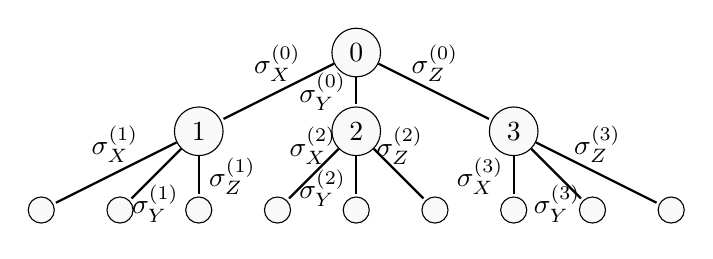
\begin{tikzpicture}[
    shorten > = 1pt,
node distance = 3cm and 4cm,
    el/.style = {inner sep=2pt, align=left, sloped},
every label/.append style = {font=\tiny}
                    ]
\node[shape=circle,draw=black,fill=gray!5] (0) at (4,2) {0}; 
\node[shape=circle,draw=black,fill=gray!5] (1) at (2,1) {1};
\node[shape=circle,draw=black,fill=gray!5] (2) at (4,1) {2};
\node[shape=circle,draw=black,fill=gray!5] (3) at (6,1) {3};
\node[shape=circle,draw=black,fill=gray!5] (4) at (0,0) {};
\node[shape=circle,draw=black,fill=gray!5] (5) at (1,0) {};
\node[shape=circle,draw=black,fill=gray!5] (6) at (2,0) {};
\node[shape=circle,draw=black,fill=gray!5] (7) at (3,0) {};
\node[shape=circle,draw=black,fill=gray!5] (8) at (4,0) {}; 
\node[shape=circle,draw=black,fill=gray!5] (9) at (5,0) {}; 
\node[shape=circle,draw=black,fill=gray!5] (10) at (6,0) {}; 
\node[shape=circle,draw=black,fill=gray!5] (11) at (7,0) {}; 
\node[shape=circle,draw=black,fill=gray!5] (12) at (8,0) {}; 



\path [-] (0) edge[color=black,thick] node[pos=0.5, above] {$\sigma^{(0)}_X$} (1);
\path [-] (0) edge[color=black,thick] node[pos=0.5, left]  {$\sigma^{(0)}_Y$} (2);
\path [-] (0) edge[color=black,thick] node[pos=0.5, above]  {$\sigma^{(0)}_Z$} (3);
\path [-] (1) edge[color=black,thick] node[pos=0.5, above] {$\sigma^{(1)}_X$} (4);
\path [-] (1) edge[color=black,thick] node[pos=0.5, below] {$\sigma^{(1)}_Y $} (5);
\path [-] (1) edge[color=black,thick] node[pos=0.5, right] {$\sigma^{(1)}_Z $} (6);
\path [-] (2) edge[color=black,thick] node[pos=0.5, above] {$\sigma^{(2)}_X$} (7);
\path [-] (2) edge[color=black,thick] node[pos=0.8, left] {$\sigma^{(2)}_Y $} (8);
\path [-] (2) edge[color=black,thick] node[pos=0.5, above] {$\sigma^{(2)}_Z $} (9);
\path [-] (3) edge[color=black,thick] node[pos=0.5, left] {$\sigma^{(3)}_X$} (10);
\path [-] (3) edge[color=black,thick] node[pos=0.5, below] {$\sigma^{(3)}_Y$} (11);
\path [-] (3) edge[color=black,thick] node[pos=0.5, above] {$\sigma^{(3)}_Z$}(12);

\end{tikzpicture}
\caption{Ternary tree structure in the case of a $4$ fermionic modes system. Labeled nodes represent qubits, while unlabeled nodes are empty and added only to complete the edges from the previous level. We note $h$ the height of the tree (here we have $h=2$). The operators are placed on edges but apply to the qubit at the origin of each edge (i.e. the qubit with index corresponding to the node from which the edge start). By convention, $X$ applies to left edges, $Y$ to central edges, and $Z$ to right edges.}
\label{fig:ternary_tree}
\end{figure}

These operators clearly obey the same anti-commutator relationships as Majorana operators: $\{ A_{\boldsymbol{p}}, A_{\boldsymbol{q}}\}= 0$ if $\boldsymbol{p} \neq \boldsymbol{q}$, and $ A_{\boldsymbol{p}}^2 = \unit$. Given there are $2n + 1$ distinct path in the ternary tree, and we need $2n$ Majorana operators, Jiang et al. \cite{Jiang2020} propose mapping each $A_{\boldsymbol{p}}$ to a single Majorana operator, and these operators have a maximum Pauli weight equal to the height of the tree ($h$), hence $\log_3(2n + 1)$. 

To construct the Hamiltonian, one needs to first transform the fermionic operators into Majorana operators and re-write the Hamiltonian, and then decide on an allocation of the Pauli operators defined above to the Majorana operators \cite{Jiang2020}. Similar to the encodings defined previously defined, the number of qubits $N$ is equal to the number of fermionic modes $n$, and the scaling of the number of Pauli operators is the same as that of the two body-terms in the second quantized Hamiltonian $\mathcal{O}(N^4)$.


\subsubsection{Discussion on generalized encondings}

Before drawing a comparison of the different generalized encodings mentioned above, we would like to raise two relevant points regarding this type of encoding: 
\begin{itemize}
    \item All the encoding mentioned above can be constructed in terms of Fenwick trees \cite{Havlek2017}, providing an opportunity to define them differently and possibly optimize the encoding to specific fermionic models. We included a description of Fenwick trees construction (similar to the presentation in Ref.~\cite{Havlek2017}) and their relation to encodings in Appendix \ref{sec:Fenwick_trees}. Fenwick trees are also relevant in the context of optimizing the Bravyi-Kitaev mapping for application to 2-dimensional lattice models \cite{Havlek2017}. 
    \item Steudtner et al. \cite{Steudtner2018} propose three additional generalized encodings which allow the number of qubits to be reduced using symmetries at the cost of additional entangling gates. Because the method presented in Ref.~\cite{bravyi_tapering_2017} and Ref.~\cite{Setia2020} addresses these symmetries without significant additional gate cost (see Sec. \ref{sec:tappering_qubits}), it is in general preferred. We nonetheless encourage readers interested in going deeper in the knowledge of these general encodings to go through Ref.~\cite{Steudtner2018} as it discusses the relevant theory in depth. 
\end{itemize}

The key metric for comparing the four mappings presented above is their Pauli weight: while Jordan-Wigner and Parity scale $\mathcal{O}(N)$, Bravyi-Kitaev scales $\mathcal{O}(\log_2(N))$ and the optimal ternary tree encoding scales $\mathcal{O}(\log_3(2N))$ (which is asymptotically the better one). The number of qubits is the same across all these mappings and equates to the number of fermionic modes ($N=n$). These mappings can also benefit from the same amount of qubit reduction using symmetries (see Sec. \ref{sec:tappering_qubits}). While the number of operators may vary, it has also been shown numerically that in general applying grouping strategies (presented in Sec. \ref{sec:Grouping}) to these operators results in a very similar number of total operators to measure \cite{Hamamura2020}. 

Because the Bravyi-Kitaev and optimal ternary tree mappings have lower Pauli weight, they are in theory less subject to read-out errors. However, this becomes invalid once the grouping of the Pauli operators for joint measurements is introduced. This is because, for most groups, the entire register of qubits needs to be measured in the $Z$ basis. The main advantage of the $\log_2(N)$ or $\log_3(Nn)$ Pauli weight is in using the mapping to construct an ansatz based on fermionic operators (such as the Unitary Coupled Cluster ansatz, UCC, see Sec. \ref{sec:UCCA}). Numerical studies looking at the use of Bravyi-Kitaev mapping in the context of Quantum Phase Estimation have consistently shown that it results in a significant reduction in the number of entangling gates required \cite{Tranter2015, Tranter2018, Setia2018}, without impacting the overall accuracy of the result in noiseless simulations. It is clear these results also translate to applications of the UCC ansatz in the context of the VQE and are likely to extend to the optimal ternary tree mapping. It is important to note that the relative impact of low Pauli weight is very much dependent on the degree of connectivity of the qubit register, and limited connectivity (e.g. qubits placed in a line), could result in a significant increase in the number of entangling gates required in a low Pauli weight encoding.

A final point to note is that a recent study \cite{Sawaya2016} numerically tested that UCC ansatz constructed for VQE with the Bravyi-Kitaev mapping could result in slightly higher sensitivity to quantum noise channels (see Appendix \ref{sec:common_noise_models}) than the Jordan-Wigner mapping, despite lower gate depth. Sawaya et al.\cite{Sawaya2016} conjecture that this could be because occupation numbers are stored locally in the Jordan-Wigner mapping: a single qubit error only impacts the result of one orbital, while for the Bravyi-Kitaev mapping, it could affect several. This also implies that occupation number errors create greater errors in the energy than parity errors \cite{Sawaya2016}. One could expect the parity and ternary tree mappings to be affected by the same phenomenon, although we are aware of any further research on this topic. 

    
\subsection{Lattice model tailored encoding} \label{sec:lattice_encoding}

The mappings defined above are oftentimes inefficient for lattice models. This is because they assume full connectivity between the different fermionic modes, and translating this into spin-operators results in non-local operations. Instead, the mappings presented in this section are concerned about being as efficient as possible for a given lattice model, where fermionic modes are attached to a specific geometry. The earliest explicit definition of fermion to qubit mapping was indeed an application to the Hubbard model \cite{Abrams1997}. The literature is divided into two mains approaches for doing so: auxiliary fermion schemes \cite{Verstraete2005, Ball2005} and Loop-Stabilized Bravyi-Kitaev (LSBK), also known as Superfast Encoding (SFE) \cite{Bravyi2002}. Maintaining low Pauli weights comes at a cost of additional qubits for all the methods mentioned in this section. However, it has been shown that all these methods also allow for at least some degree of error correction. A summary of the key metrics of each encoding is presented in Table~\ref{tab:lattice_encoding}.

\begin{table} [ht]
\caption{Comparative summary of lattice tailored encodings. $d$ represents the degree of the Hamiltonian graph, $v$ and $h$ respectively the vertical and horizontal dimensions of a 2-dimensional lattice (we set $v \leq h$), $n$ is the number of fermionic modes / sites on the lattice. The number of operators scales linearly with $E$, the number of edges. We have $E = h(v - 1) + v (h - 1)$ for a 2-dimensional regular lattice, and $E = \sum_i^D \left[ (n_i - 1) \prod_{j \neq i}^D n_j \right]$ for an regular lattice of dimension $D$ and $n_i$ the number of sites along the $i^{th}$ dimension.} \label{tab:lattice_encoding}
\begin{tabularx}{\linewidth}{X|m{0.15\linewidth}m{0.15\linewidth}X}
\toprule
Method &  Pauli Weight & Qubits & Comments \\
\midrule
    Jordan-Wigner (snake pattern) \cite{Verstraete2005} & $\mathcal{O}(2v)$ & $n$ & Optimal direct application of the Jordan-Wigner mapping to a 2-dimensional lattice.  \\\\
\hline\\
    Bravyi-Kitaev (Fenwick tree lattice mapping) \cite{Havlek2017} & $\mathcal{O}(\log(v))$ & $n$ & Optimal direct application of the Bravyi-Kitaev mapping to a 2-dimensional lattice.  \\\\
\hline\\
    Auxiliary Fermion Scheme \cite{Verstraete2005} & $4$ (2-dim.) & $2n$, ($n = vh$) & Uses auxiliary fermion/qubit registers to create operators that cancel-out $Z$ strings in the Jordan-Wigner mapping  \\\\
\hline\\
    Superfast Bravyi-Kitaev \cite{Bravyi2002, Havlek2017, Setia2018} & $\mathcal{O}(2d)$& $\mathcal{O}(nd/2)$ & Relies on stabilizers formalism to define an efficient encoding with cost dependent on the degree of the Hamiltonian graph  \\\\
\hline\\
    Generalized Superfast Encoding \cite{Setia2019} & $\mathcal{O}(\log_2(d))$ & $\mathcal{O}(nd/2)$ &Extension of Superfast BK, optimizing Pauli weight and offering better opportunities for error corrections  \\\\
\hline\\
    Compact encoding \cite{Derby2021, Derby2021_part2} & $3$ (2-dim.), $4$ (3-dim.) & $\mathcal{O}(1.5n)$ &Modifies the stabilizer formalism used in Superfast BK to optimize the number of qubits required. So far limited to 2 and 3-dimensional lattices \\\\
\bottomrule
\end{tabularx}
\end{table}

All the mappings presented in this section will exhibit a similar scaling in the number of operators produced, which will be linearly proportional to the number of edges $E$ in the lattice. For example, consider a regular lattice of dimension $D$, with $n_i$ the number of sites along the $i^{th}$ dimension we easily obtain
\begin{equation}
    E = \sum_i^D \left[ (n_i - 1) \prod_{j \neq i}^D n_j \right].
\end{equation}
We also have the total number of sites $n = \prod_{j}^D n_j$ and therefore a number of edges is capped below $\mathcal{O}(nD)$. An additional pre-factor should be included to account for the fact that some encoding require auxiliary sites (and hence auxiliary operators), however this does not change the overall scaling.


\subsubsection{Auxiliary fermion schemes}

Suppose a 1-dimensional spin-chain, with only nearest neighbor interactions. All operators of interest are of the form $\hat{a}_i^{\dagger}\hat{a}_j$, with $i = j \pm 1$. Therefore, under the Jordan-Wigner mapping all operators have the form
\begin{equation} \label{eq:hopping}
\hat{a}_{i \pm 1}^{\dagger} \hat{a}_{i}=\frac{X_{i \pm 1}-i Y_{i \pm 1}}{2} \otimes \frac{X_{i}+i Y_{i}}{2}.
\end{equation}
One can note that the $Z$ strings required to maintain the anticommuting relationship have canceled out, and are no longer necessary: the Jordan-Wigner mapping preserves operator locality in one-dimensional systems. Auxiliary Fermion Schemes answer the question of how to maintain operator locality in mappings such as Jordan-Wigner when the lattice model considered has higher dimensions.  

A first example of encoding tailored for lattice model was independently proposed in \cite{Verstraete2005} and \cite{Ball2005}. As described above (both grounded in \cite{Levin2003, Wen2003}), it can be seen as a Jordan-Wigner encoding optimized for rectangular lattice problems. It avoids the need for strings of $Z$ operators in interaction terms built out of creation and annihilation operators thereby optimizing the Pauli weight, but at the cost of increasing the number of qubits. This is referred to in the literature alternatively as the Ball-Verstraete-Cirac (BVC) encoding (for example \cite{Whitfield2016}.

Suppose a rectangular spin lattice, such as the 2-dimensional Hubbard model. One could nearly map it to a one-dimensional system by ordering the operators (for example, as the 'snake pattern' presented in Fig. \ref{fig:nine_site_lattice}). Along with this ordering (i.e. considering only the operator connections it covers), one can easily implement a local version of the Jordan-Wigner mapping. The issue however is that some connections are not covered and cannot be directly expressed with local operators using the Jordan-Wigner mapping (consider for example the dotted line between site 1 and 6, representing operators $\hat{a}^{\dagger}_1 \hat{a}_6$ and transpose in the figure, which would require $Z$ strings in this ordering).

\begin{figure} [h]
\centering
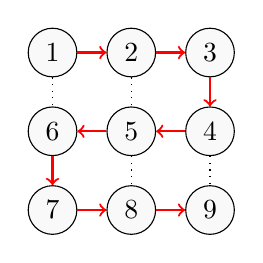
\begin{tikzpicture}
\node[shape=circle,draw=black,fill=gray!5] (1) at (0,2) {1}; 
\node[shape=circle,draw=black,fill=gray!5] (2) at (1,2) {2};
\node[shape=circle,draw=black,fill=gray!5] (3) at (2,2) {3};
\node[shape=circle,draw=black,fill=gray!5] (6) at (0,1) {6};
\node[shape=circle,draw=black,fill=gray!5] (5) at (1,1) {5};
\node[shape=circle,draw=black,fill=gray!5] (4) at (2,1) {4};
\node[shape=circle,draw=black,fill=gray!5] (7) at (0,0) {7};
\node[shape=circle,draw=black,fill=gray!5] (8) at (1,0) {8};
\node[shape=circle,draw=black,fill=gray!5] (9) at (2,0) {9}; 

\path [->] (1) edge[color=red,thick] (2);
\path [->] (2) edge[color=red,thick] (3);
\path [->] (3) edge[color=red,thick] (4);
\path [->] (4) edge[color=red,thick] (5);
\path [->] (5) edge[color=red,thick] (6);
\path [->] (6) edge[color=red,thick] (7);
\path [->] (7) edge[color=red,thick] (8);
\path [->] (8) edge[color=red,thick] (9);
\path [-] (1) edge[color=black,dotted] (6);
\path [-] (2) edge[color=black,dotted] (5);
\path [-] (5) edge[color=black,dotted] (8);
\path [-] (4) edge[color=black,dotted] (9);

\end{tikzpicture}
\caption{Example of a 2-dimensional spin lattice with nine sites. Edges represent connections between the different fermionic modes. Red arrows are connections that provide an example of a 'snake ordering' of the fermionic modes in a 1-dimensional pattern, while dotted lines show the connections missed by the ordering.}
\label{fig:nine_site_lattice}
\end{figure}

The BVC mapping provides a means to encode operators along the edges not covered in the ordering locally. In order to do so, it defines an auxiliary Hamiltonian composed of a weighted sum or interaction operators which are constructed using an alternative set of fermionic operators $\hat{b}_i$ such that
\begin{equation}
    \hat{\mathcal{H}}_{\mathrm{aux}} = \sum_{\{i, j\}} \hat{h}_{ij}^{(\mathrm{aux})} = \sum_{\{i, j\}} - (\hat{b}_i + \hat{b}_i^{\dagger})(\hat{b}_j - \hat{b}_j^{\dagger}), 
\end{equation}
which we note can be re-written in terms of Majorana operators (see Eq. \ref{eq:majorana}): 
\begin{equation}\label{eq:auxiliary_couplings}
    \hat{\mathcal{H}}_{\mathrm{aux}} = \sum_{\{i, j\}} i \hat{\gamma}_i \hat{\gamma}_{j+1}. 
\end{equation}

The fermions are configured to be in the ground state of this Hamiltonian, denoted $\ket{\chi}$. The auxiliary Hamiltonian sites match those of the physical Hamiltonian. The overall system is now composed of $2n$ fermions which we can order as $1, 1^{\prime}, 2, 2^{\prime}, \dots n, n^{\prime}$.   

For notational simplicity, indices of the auxiliary fermionic system are primed. From there, the edges of the physical lattice Hamiltonian which are not covered by the initial ordering of fermions into a 1-dimensional system (indexed here by $\{p, q \}$), can be modified as follows:

\begin{equation}
    \hat{a}^{\dagger}_p\hat{a}_q \rightarrow \hat{a}^{\dagger}_p\hat{a}_q \hat{h}_{pq}^{(\mathrm{aux})} = \hat{a}^{\dagger}_p\hat{a}_q \left(i \hat{\gamma}_{p^{\prime}} \hat{\gamma}_{q^{\prime} + 1} \right).
\end{equation}

It is important to note, that because any of the vertical hopping terms in the physical Hamiltonian commute with the auxiliary Hamiltonian, the operation described above does not modify the ground state of the system. The consequence is that when now applying the Jordan-Wigner transformation to the new, joint Hamiltonian, the $Z$ strings of the original, non-covered edges are canceled out by those of the auxiliary terms by which they have been modified. Note that using Jordan-Wigner, the auxiliary Hamiltonian presented in Eq. (\ref{eq:auxiliary_couplings}) can be non-local, though this can be addressed easily by substitution of the non-local operators with local ones (see Ref.~\cite{Verstraete2005} for details).
The main advantage of this method is that, as long as only nearest-neighbor interactions are allowed, it caps the Pauli weights to 4 for hopping terms (basically following Eq.~\ref{eq:hopping}), and to $2$ for Coulomb terms. Suppose a rectangular lattice of $h \times v$ sites, (we set $v \leq h$), a naive implementation of a Jordan-Wigner mapping would result in a maximum Pauli weight of $\mathcal{O}(2v)$ (consider for example the mapping of the hopping term between site 1 and 6 in Fig. \ref{fig:nine_site_lattice}). This benefit comes at the cost of doubling the number of qubits required due to the introduction of the auxiliary Hamiltonian, hence a total of $2vhL$ qubits as initially one is required for each fermionic mode.   

Whitfield {\it et al.} \cite{Whitfield2016} extend the theory of the BVC mapping presented in \cite{Verstraete2005, Ball2005}, by showing that there is a range of possible choices of the auxiliary coupling operators, which are not required to be Majorana operators. They also show that the number of auxiliary modes required for each fermionic mode in a lattice grows as $D - 1$, with $D$ the dimension of the lattice. Further improvements were also proposed in \cite{Steudtner2019}.

An adaptation of the auxiliary fermion scheme to the Bravyi-Kitaev encoding is also proposed by Havl{\'{\i}}{\v{c}}ek {\it et al.} ~\cite{Havlek2017}, thereby optimizing it for rectangular lattice models. Havl{\'{\i}}{\v{c}}ek {\it et al.} propose to first build the Bravyi-Kitaev mapping into a data structure using a Fenwick tree and then map the connections of this Fenwick tree to a fermion lattice. Because sites that are connected through the tree (either by mean of the parity set or the update set) only require local operations, non-local operations are restricted to the mapping of connections on the lattice which are not included on the tree. By doing so, they show that with optimal mapping of the Fenwick tree to the lattice, the Pauli weight of their adapted Bravyi-Kitaev encoding scales as $\mathcal{O}(\log(v))$, with $v$ the smallest side of the lattice. 


\subsubsection{Superfast Encoding / Loop Stabilizer Encodings} \label{sec:superfast_encoding}
The encoding concept developed in this section was initially presented in \cite{Bravyi2002} and is based on a graph representation of the Hamiltonian. Of course, any lattice models (or \textit{ab initio} molecular system) can be represented as a graph, where each fermionic mode is a vertex, and each interaction with another fermionic mode is a weighted edge in the graph. Unlike the mappings presented so far, in this mapping, qubits are used to encode interactions between fermionic modes rather than the state of the fermionic modes themselves. It is referred to in the literature as the Superfast Bravyi-Kitaev (SFBK) or alternatively, Loop-Stabilized Bravyi-Kitaev (LSBK) \cite{Havlek2017} (we use SFBK as it is more generally used in the literature).

The overall advantage of this method is that, similar to the auxiliary qubit scheme, the Pauli weight of the qubit operators corresponding to the fermionic operators does not depend on the number of fermionic modes in the Hamiltonian but instead depends on the degree of the interaction graph. The number of qubits required depends on the total number of edges which is a function of the total number of fermionic modes and the degree of the interaction graph. This makes Superfast Encoding more suitable for lattice based models. We first present the SFBK mapping, as theorized in \cite{Bravyi2002}, and further developed in \cite{Whitfield2016, Havlek2017, Setia2018}, and we then turn to extensions developed based on this encoding \cite{Setia2019, Jiang2019, Derby2021, Derby2021_part2}.

\paragraph{Background and definition of SFBK:}
Given the fermionic Hamiltonian an interaction graph can be constructed. The set of edges, $E$ for the interaction graph correspond to the excitation, number excitation and double excitation operators (e.g. Fig. \ref{fig:h2moleculegraph1}). In SFBK, the qubits are placed on the edges of the interaction graph, and the Fock space of the fermionic modes is associated with a codespace of a stabilizer code defined on the qubits on the edges. The qubit indices are defined based on two fermionic indices where a connection exists (e.g. $(jk)$). To define the codespace and the fermionic operators in terms of the qubit operators acting on qubits on the edges of the interaction graph, it is helpful to work with the Majorana modes defined in terms of Fermionic modes as in Eq. (\ref{eq:majorana}). These operators are Hermitian and satisfy
\begin{align}
\hat{\gamma}_{j}\hat{\gamma}_{k}+\hat{\gamma}_{k}\hat{\gamma}{j}=2\delta_{jk} \label{eq:Maj_modes}
\end{align}
Using Majorana modes, the following vertex operator and edge operator can be defined as
\begin{equation}
\begin{aligned}
\hat{B}_j &= -i \hat{\gamma}_j\hat{\gamma}_{j+1}, \quad
\hat{A}_{jk} &= -i\hat{\gamma}_j\hat{\gamma}_k.
\end{aligned}
\end{equation}
The vertex operator $\hat{B}_j$ only acts on fermionic mode $j$, while the edge operator $\hat{A}_{jk}$ connects fermionic mode $j$ to mode $k$. These operators satisfy the following algebraic relations:
\begin{align} \label{eq:algebra_sfbk_bb}
&\left[ \hat{B}_k, \hat{B}_l \right] = 0,\\
&\hat{A}_{(jk)}\hat{B}_l = (-1)^{\delta_{(jl)} + \delta_{(kl)}} \hat{B}_l \hat{A}_{(jk)}, \label{eq:algebra_sfbk_ab} \\
&\hat{A}_{(jk)}\hat{A}_{(ls)} =  (-1)^{\delta_{(jl)} + \delta_{(js)} + \delta_{(kl)} + \delta_{(ks)}}\hat{A}_{(ls)}\hat{A}_{(jk)}, \label{eq:algebra_sfbk_aa}
\end{align}
and the loop condition:
\begin{align} \label{eq:sfbk_loop}
(i)^{p} \hat{A}_{(j_0 j_1)}\hat{A}_{(j_1 j_2)} \dots \hat{A}_{(j_{p-1} j_p)}\hat{A}_{(j_p j_0)} = \unit,
\end{align}
with $j_0 \dots j_p$ any closed loop over the vertex indices.

It can be shown that the vertex and the edge operators satisfying the above relations generate the algebra of the physical operators. This means that any physical Hamiltonian with even fermionic modes can be represented in terms of these edge and vertex operators. The fermionic creation and annihilation operators can be converted into Majorana modes which can then be converted to edge and vertex operators. Table \ref{tab:SFBKoperatortable} gives the edge and vertex operators expressions for various Hamiltonian terms (with computation initially presented in \cite{Setia2018}). 
\begin{figure} [h]
\centering
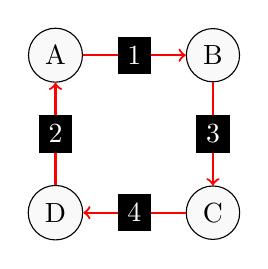
\begin{tikzpicture}
\node[shape=circle,draw=black,fill=gray!5] (D) at (0,0) {D};  \node[shape=circle,draw=black,fill=gray!5] (A) at (0, 2) {A};
\node[shape=circle,draw=black,fill=gray!5] (B) at (2, 2) {B};
\node[shape=circle,draw=black,fill=gray!5] (C) at (2, 0) {C};

\path [->] (A) edge[color=red,thick] (B);
\path [->] (B) edge[color=red,thick] (C);
\path [->] (C) edge[color=red,thick] (D);
\path [->] (D) edge[color=red,thick] (A);

\node[shape=rectangle, draw=black,fill=black, text=white] (4) at (1, 0) {4};
\node[shape=rectangle,draw=black,fill=black, text=white] (2) at (0, 1) {2};
\node[shape=rectangle,draw=black,fill=black, text=white] (1) at (1, 2) {1};
\node[shape=rectangle,draw=black,fill=black, text=white] (3) at (2, 1) {3};
\end{tikzpicture}
\caption{A graph corresponding to the SFBK encoding defined from the $H_2$ Hamiltonian in a minimal basis set: fermions in the physical system of interest correspond to the vertices (grey circles) of the graph; qubits (the black rectangles) in the quantum computer are associated to the edges (red arrows) on the graph; the vertices and edges the graph are used to define the edge and vertex fermionic operators $\hat{A}_{jk}$ and $\hat{B}_j$, which in turn correspond to edge and vertex qubit operators $\tilde{A}_{jk}$ and $\tilde{B}_j$}
\label{fig:h2moleculegraph1}
\end{figure}
Using the algebraic relations for the edge and vertex operators we can define the qubit operators for the edge and vertex operators. As we will see through the construction, it is also possible to define the codespace for the simulation.

Starting from the vertex operator, we note that $\hat{B}_k$ obeys an additional constraint on the excitation parity when considering an even number of fermions in the system, for a total of $\mathrm{V}$ vertices, the fermion parity operator is

\begin{equation} \label{eq:vertex_sfbk}
\begin{aligned}
\prod_{k \in \mathrm{V}} \hat{B}_k = \unit
\end{aligned}
\end{equation}

If the number of particles is instead odd, one can always split the Hamiltonian in even and odd sectors, the odd sector can be simulated by changing the sign of the mapping as described below in Eq.~(\ref{eq:vertex_sfbk_qubit}) \cite{Jiang2019}. From Eq. \ref{eq:vertex_sfbk} and the rule defined in  Eq.~(\ref{eq:algebra_sfbk_bb}), one can easily create a corresponding definition for the qubit version vertex operator $\tilde{B}_k$:
\begin{equation}\label{eq:vertex_sfbk_qubit}
\tilde{B}_{k} =\bigotimes_{j \in n(k)} Z_{(k j)},
\end{equation}
where $n(j)$ is the set of vertices connected to mode $j$ by an edge, and the pair $(kj)$ indexes a qubit. This definition meets the constraint of Eq. \ref{eq:vertex_sfbk} as each edge is connected to exactly two vertices. We note that the Pauli weight for these operators is capped at the degree of the Hamiltonian graph. 

For the edge operator $\hat{A}_{(jk)}$, we start by defining an ordering of the vertices and related direction of edges, such that $\epsilon_{jk} = 1$ when $j > k$, and $\epsilon_{kj} = - 1$. Looking first at the rule of Eq.~(\ref{eq:algebra_sfbk_ab}), in the case where $l \neq j$ and $l \neq k$ operators $\hat{A}_{(jk)}$ and $\hat{B}_{l}$ must commute, and hence given the definition of $\tilde{B}_{l}$ from Eq.~(\ref{eq:vertex_sfbk_qubit}) all qubit operators representing edges adjacent to $j$ or $k$ (except for $(jk)$ itself) must be either $\unit$ or $Z$, as $l$ could be one of the connected vertices. 
If $l = j$ or $k$, then $\hat{A}_{(jk)}$ and $\hat{B}_{l}$  must anticommute. Following the same reasoning as above, the qubit operator on the edge connecting $l$ to the other vertex ($j$ or $k$) must anticommute with $Z$: it must be either $X$ or $Y$. 

The last commutation rule that must be met is Eq.~(\ref{eq:algebra_sfbk_aa}), which states that two edge operators anticommute if they share a single vertex (they commute otherwise). All these conditions, together can be met by the following qubit operator as defined in \cite{Bravyi2002, Havlek2017, Setia2018}:
\begin{equation}
\tilde{A}_{(j k)} =\epsilon_{j k} X_{(j k)} \bigotimes_{l < k}^{n(j)} Z_{(l j)} \bigotimes_{s < j}^{n(k)} Z_{(s k)},
\end{equation}
where the $Z$ operators on vertices either connected and directed into $j$ or from $k$, and the $X$ operator on vertex $(jk)$ enforce the rule of Eq.~(\ref{eq:algebra_sfbk_ab}), and the phase factor $\epsilon_{j k}$ enforce the rule of Eq.~(\ref{eq:algebra_sfbk_aa}).

The qubit operator representation of vertex and edge operators $\tilde{B}_{j}$ and $\tilde{A}_{(j k)}$ do not satisfy the loop condition defined in Eq.~(\ref{eq:sfbk_loop}). And this condition lets us define the codespace. Using the qubit operator representation of the edge operator, $\tilde{A}_{jk}$, we can define a set of stabilizers corresponding to the loops in the graph and define the codespace to be the subspace where the loop condition defined in Eq.~(\ref{eq:sfbk_loop}) hold. The loop operator is defined as follows:
\begin{equation} \label{eq:loop_operator}
    \tilde{A}(\eta) \equiv  (i)^{p} \hat{A}_{(\eta_0 \eta_1)}\hat{A}_{(\eta_1 \eta_2)} \dots \hat{A}_{(\eta_{p-1} \eta_p)}\hat{A}_{(\eta_p \eta_0)}, 
\end{equation}
with $\eta$ defining a loop of length $p$ on the Hamiltonian graph. 
This definition of the loop operator generates an Abelian group of all the stabilizers (all necessary properties of this group are explored and demonstrated in \cite{Setia2019}). The number of independent loops $s$ in the graph is equal to the number of edges, minus the number of vertices plus one, or recalling $N$ the number of qubits, and $n$ the number of fermionic mode: $s = N - n + 1$. Therefore the code space defined by the stabilizer group encodes $N - s = n - 1$ logical qubits, into $N$ physical qubits. This code space effectively restricts operators to the even parity subspace of the fermionic Fock space \cite{Bravyi2002, Setia2019}. Once this restriction is applied to $\hat{B}_{j}$ and $\hat{A}_{(j k)}$, one can defined an encoded qubit Hamiltonian.

The total number of qubits required for this encoding is proportional to the number of edges in the Hamiltonian graph. For regular lattice models, the number of edges itself is a direct multiple of the graph degree and of the number of sites. Since the Pauli weight of vertex and edge operators scales as $O(d)$, where $d$ is the degree of the interaction graph, the Pauli weight of each term in the transformed Hamiltonian also scales as $O(d)$.


\begin{table*}
\caption{Molecular Hamiltonian operators in second quantized form and in the corresponding vertex and edge operator form used in the Superfast Bravyi-Kitaev encoding.}
\begin{tabular}{ l | cc}
  \toprule			
Operator & Second quantized form & Vertex and edge operator form \\    \midrule
Number operator & $h_{pp} \hat{a}_p^\dagger \hat{a}_p$ & $\frac{1 - \hat{B}_p}{2}$ \\ 
Coulomb/exchange operators & $h_{pqqp} \hat{a}_p^\dagger \hat{a}_q^\dagger \hat{a}_q \hat{a}_p$ & $h_{pqqp} \frac{(1 - \hat{B}_p)(1 - \hat{B}_q)}{4}$ \\ 
Excitation operator & $h_{pq} (\hat{a}_p^\dagger \hat{a}_q + \hat{a}_q^\dagger \hat{a}_p$) & $-h_{pq} \frac{i}{2} (\hat{A}_{pq} \hat{B}_q + \hat{B}_p \hat{A}_{pq}) $ \\  
Number-excitation operator & $h_{pqqr} (\hat{a}_p^\dagger \hat{a}_q^\dagger \hat{a}_q \hat{a}_r + \hat{a}_r^\dagger \hat{a}_q^\dagger \hat{a}_q \hat{a}_p)$ & $- h_{pqqr} \frac{i}{4} (\hat{A}_{pr} \hat{B}_r + \hat{B}_p \hat{A}_{pr}) (1 - B_q) $ \\  
Double excitation operator & $h_{pqrs} (\hat{a}_p^\dagger \hat{a}_q^\dagger \hat{a}_r \hat{a}_s + \hat{a}_s^\dagger \hat{a}_r^\dagger \hat{a}_q \hat{a}_p)$ & $\frac{h_{pqrs}}{8} \hat{A}_{pq} \hat{A}_{rs} (-1 - \hat{B}_p \hat{B}_q + \hat{B}_p \hat{B}_r +$ \\ && $\hat{B}_p \hat{B}_s + \hat{B}_q \hat{B}_s - \hat{B}_r \hat{B}_s - \hat{B}_q + \hat{B}_p \hat{B}_r \hat{B}_s)$\\
  \bottomrule	
\end{tabular}
\label{tab:SFBKoperatortable}
\end{table*}

SFBK was applied to the 2-dimensional Hubbard model in Ref.~\cite{Havlek2017} and was shown to be applicable to \textit{ab initio} molecular systems in \cite{Setia2018}. In both cases, it is clear that for a Hamiltonian graph of degree $d$, and a number of fermionic modes $n$, the Pauli weight of SFBK scales $\mathcal{O}(2d)$ and the number of qubits required scales $\mathcal{O}(nd/2)$.

\paragraph{Generalized Superfast Encoding:}
The Abelian stabilizer group defined using the loop operators given in Eq.~(\ref{eq:loop_operator}) defines the codespace for the simulation. Since the edge and vertex operators commute with the stabilizer group, a state initialized within the codespace remains in codespace through the action of edge or vertex operators. Any operation that moves the state out of the codespace is not valid and can be considered as an error. 
The motivation for the Generalized Superfast Encoding was to come up with a modified version of SFBK that can detect all the errors. The number of qubits required for GSE is the same as SFBK, but the Pauli weight of qubit operator representation of edge and vertex operator is lower and scales as $\mathcal{O}(\log(d))$.

In contrast to SFBK, where qubits are placed on the edges, GSE places them on vertices which consequently modifies the operators used for the encoding. For each fermionic mode $j$ (which are assumed to be even in GSE), one must use $d^{(j)}/2$ qubits, where $d^{(j)}$ is the degree of the vertex corresponding to the mode $j$. Hence, it has the same scaling of the number of qubits as for SFBK: $\mathcal{O}(nd/2)$.

In the GSE, a vertex $j$ with $d/2$ qubits encodes $d$ Majorana modes $\hat{\gamma}{j, 1}, \hat{\gamma}{j, 2},...\hat{\gamma}{j, d}$. A procedure to construct these Majorana modes can be found in \cite{Setia2018}. The vertex and edge operator for qubits can be reformulated for the GSE as follows: 
\begin{equation}\label{eq:vertex_gse_qubit}
\tilde{B}_{j} = (-i)^{d^{(j)}/2}\hat{\gamma}{j, 1}\hat{\gamma}{j, 2} \dots\hat{\gamma}{j, d^{(j)}},
\end{equation}
\begin{equation} \label{eq:edge_gse_qubit}
\tilde{A}_{(j k)} =\epsilon_{j k} \hat{\gamma}{j, p} \hat{\gamma}{k, q},
\end{equation}
where $p$ is the $p$-th local Majorana mode on the site $j$, and $q$ is the $q$-th local Majorana mode on the site $k$.  These operators can also be restricted to the even-partiy subspace, using the same stabilizers  definition based on the loop operator of Eq.~(\ref{eq:loop_operator}) \cite{Setia2019}. It can be shown using Fenwick tree encoding \cite{Havlek2017} (see appendix \ref{sec:Fenwick_trees}) that a Majorana mode $\hat{\gamma}{j, p}$ can be encoded into Pauli operators of weight $\log_2 d^{(j)}$. This means that operators $\tilde{A}_{(j k)}$ of Eq.~(\ref{eq:edge_gse_qubit}) have a maximum Pauli weight of $2\log_2 d$, while operators $\tilde{B}_{j}$ (Eq. \ref{eq:vertex_gse_qubit}) have a Pauli weight of $1$ as it requires a single $Z$ string \cite{Havlek2017}. This shows a key advantage of GSE over SFBK. 

As mentioned above, it is shown in \cite{Setia2019} that GSE additionally allows use of the code space defined as part of the encoding as a means of performing error correction. This property is applicable from $ d^{(j)} \geq 6$ and catches single-qubit errors. So far, the error threshold tolerance of this error mitigation method has not been estimated.

Setia {\it et al.} \cite{Setia2019} also showed that SFBK cannot provide single-qubit error correction for Hamiltonian graph of degree $ d^{(j)} \leq 6$.  The Majorana Loop Stabilizer Code (MLSC) was introduced in \cite{Jiang2019} as a means to allow addressing single-qubit errors on 2D square lattices (hence with vertex degree equal to $4$) while preserving a local encoding. This encoding is still dependent on further research to be extended to higher-dimensional systems. These ideas have been further generalized in \cite{Chien2020}.    

\paragraph{Compact mappings:}

The so-called compact mapping \cite{Derby2021} is another extension of SFBK which does not concern itself error correcting properties, but focuses on minimizing the Pauli weight while reducing the number of qubits required in the methods previously mentioned. Derby and Klassen \cite{Derby2021} present application of the method to square and hexagonal lattices, and extend it in  Ref.~\cite{Derby2021_part2} to uniform lattices of degree less than $4$ and cubic lattices. 

In the compact encoding, one must first assign a qubit to each vertex $j$. In a 2D lattice, each square of four vertices (referred to as a face), is defined as even or odd in a checkerboard pattern. Edges also need to be given an orientation. The orientation recommended in Ref.~\cite{Derby2021_part2} is to set the orientation anticlockwise for even faces of the lattice, orientation on odd faces follows from completion. A schematic is presented in Fig. \ref{fig:compact_encoding}.

\begin{figure} [h]
\centering
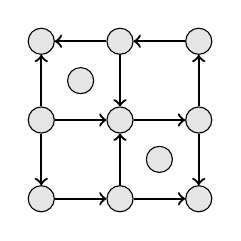
\begin{tikzpicture}
\node[shape=circle,draw=black,fill=black!10] (1) at (0,2) {}; 
\node[shape=circle,draw=black,fill=black!10] (2) at (1,2) {};
\node[shape=circle,draw=black,fill=black!10] (3) at (2,2) {};
\node[shape=circle,draw=black,fill=black!10] (4) at (0,1) {};
\node[shape=circle,draw=black,fill=black!10] (5) at (1,1) {};
\node[shape=circle,draw=black,fill=black!10] (6) at (2,1) {};
\node[shape=circle,draw=black,fill=black!10] (7) at (0,0) {};
\node[shape=circle,draw=black,fill=black!10] (8) at (1,0) {};
\node[shape=circle,draw=black,fill=black!10] (9) at (2,0) {}; 

\node[shape=circle,draw=black,fill=black!10] (10) at (0.5,1.5) {}; 
\node[shape=circle,draw=black,fill=black!10] (11) at (1.5,0.5) {}; 

\path [->] (2) edge[color=black,thick] (1);
\path [->] (4) edge[color=black,thick] (1);
\path [->] (4) edge[color=black,thick] (5);
\path [->] (2) edge[color=black,thick] (5);
\path [->] (3) edge[color=black,thick] (2);
\path [->] (5) edge[color=black,thick] (6);
\path [->] (6) edge[color=black,thick] (3);
\path [->] (4) edge[color=black,thick] (7);
\path [->] (7) edge[color=black,thick] (8);
\path [->] (8) edge[color=black,thick] (5);
\path [->] (8) edge[color=black,thick] (9);
\path [->] (6) edge[color=black,thick] (9);

\end{tikzpicture}
\caption{Example of qubit placement and edge orientation in the compact mapping. Each gray dot represents a qubit, only those connected by edges correspond to sites, the others correspond to odd lattice faces.}
\label{fig:compact_encoding}
\end{figure}

From this allocation of qubits, we can already see that the number of qubits for this encoding is capped to $1.5$ times the number of sites (or number of fermionic mode, $n$). We first define the edge operators: for a given edge $(i, j)$, oriented $i$ to $j$, at most one of the adjacent faces is odd, in which case we index the related qubit with $(i, j)$. We have for a downward edge  \begin{equation}
    \tilde{A}_{(ij)} = X_i Y_j X_{(i,j)},
\end{equation}
for an upward edge: 
\begin{equation}
    \tilde{A}_{(ij)} = - X_i Y_j X_{(i,j)},
\end{equation}
and for a horizontal edge:
\begin{equation}
    \tilde{A}_{(ij)} = X_i Y_j Y_{(i,j)}.
\end{equation}
When the edge is on a boundary of the lattice with no odd face adjacent, there is no qubit $(i,j)$, and therefore the relevant Pauli operator can be omitted. 

Vertex operators are defined as
\begin{equation}
    \tilde{B}_{j} = Z_j.
\end{equation}
It is easy to verify that these operators meet the conditions set for SFBK in Eq.~(\ref{eq:algebra_sfbk_bb}), \ref{eq:algebra_sfbk_ab}, and \ref{eq:algebra_sfbk_aa}. As for SFBK, the loop condition in Eq.~(\ref{eq:sfbk_loop}) must also be met. The key feature of the compact mapping is that it does so in a way that allow to avoid the parity condition set by Eq.~(\ref{eq:vertex_sfbk}), and with it the need to have a Pauli weight equal to the degree of the graph. 

Considering first the stabilizers for odd faces, defining $a,b,c, d$ as the four vertices (for instance consider the first face in Fig. \ref{fig:compact_encoding}), we have 
\begin{align}
    \tilde{A}_{(ab)} & = (X_bY_aY_{(a,b)}) \\ \nonumber
    \tilde{A}_{(bc)} & = (X_bY_cX_{(b,c)}) \\ \nonumber
    \tilde{A}_{(cd)} &=  (X_dY_cY_{(c,d)}) \\ \nonumber
    \tilde{A}_{(dc)} &= (-X_dY_aX_{(d,a)})   \\ \nonumber
    \tilde{A}_{(ab)}\tilde{A}_{(bc)}\tilde{A}_{(cd)}\tilde{A}_{(dc)} &= - (Y_{(a,b)}X_{(a,b)})(Y_{(a,b)}X_{(a,b)}) \\ \nonumber
    & = - (-iZ_{(a,b)})(-iZ_{(a,b)}) \\ \nonumber
    &= \unit
\end{align}
as of course, the qubit with index $(a, b)$, is the same as with index $(b, c)$, $(c, d)$, and $(d, a)$.

For even faces however, the stabilizers are non-trivial and therefore impose a constraint on the operators. Construction of these constraints are detailed in \cite{Derby2021, Derby2021_part2}. Extensions of this method to other uniform lattices of degree up to 4 and cubic lattices can be found in \cite{Derby2021_part2}. In addition, it was shown in \cite{Bausch2020} that the compact encoding can also be used to detect a large proportion of single-qubit errors. 

\subsubsection{Discussion on lattice tailored encodings}

There are three main metrics that are worth discussing when comparing the different lattice tailored mapping: the number of qubits they require, their Pauli weights, and their capacity to mitigate or even correct errors resulting from quantum noise. 

The number of qubits required appears to be a trade-off for the two other features mentioned above. All mappings from this section considered, the compact encoding from Ref.~\cite{Derby2021} offer the most advantageous combination of low number of qubits and low Pauli weights for systems of dimensions up to $3$. Extension of the compact encoding to higher dimensions requires further research. In the meantime, the GSE \cite{Setia2019} provides the best performance in terms of Pauli weight but does require that the number of qubits increases linearly with the degree $d$ of the graph (recalling $d = 2D$) and the number of sites $n$.

While we found no comprehensive studies on the matter, these would very likely result in the most compact ansatz. However, as noted in \cite{Sawaya2016} when comparing the Jordan-Wigner and Bravyi-Kitaev mappings, lower gate depth does not necessarily translate to an overall higher resilience to quantum noise.  

An overall question that remains pending regarding all the lattice mappings considered is their efficacy at realizing error mitigation or error correction. For example, while the GSE demonstrates some error correcting properties, it is still unclear what quantum noise threshold is tolerable for these properties to be useful. In particular, such assessment is required to fully compare these encoding like-for-like. For example, the compact encoding could require additional quantum resources from error mitigation techniques (see Sec. \ref{sec:error-mit}) to achieve an accuracy comparable to what can be achieved when relying on the error correcting properties of other mappings such as SFBK or GSE. 

This point also extends to applications of methods to \textit{ab initio} molecular systems. Ref.~\cite{Setia2018} shows that SFBK results in lower gate depth than Jordan-Wigner, but higher than Bravyi-Kitaev on a small molecular system. Chien \textit{et al.} \cite{Chien2019} also show that Jordan-Wigner can outperform SFBK in terms of gate count under certain conditions on the Hamiltonian studied. One can expect GSE to perform better due to its lower Pauli weight, however for a relevant comparison, one would need to incorporate equivalent error mitigation techniques into Jordan-Wigner or Bravyi-Kitaev to balance quantum resources required to achieve a given accuracy. Overall, the question of the real impact of the error mitigating and correcting properties of lattice tailored encodings could be critical in determining their future applicability. 

\subsection{Reducing qubit requirements} \label{sec:tappering_qubits}

Several methods have focused on reducing the overall number of qubits required to encode a specific Hamiltonian \cite{Moll2016, bravyi_tapering_2017, Steudtner2018, Setia2020, Kirby2021_CSVQE}. These methods usually come at limited additional costs and can therefore be used to significantly improve the efficiency of VQE. Bravyi {\it et al.} \cite{bravyi_tapering_2017}] formulate several proposals designed to reduce (`taper off') the number of qubits required to simulate fermionic systems for variational quantum algorithms. In particular, they find that it is possible to reduce qubit requirements in encodings where $\mathbb{Z}_2$ symmetries are present. This results in halving the dimension of the Hilbert space of the system considered for each qubit removed. The starting point of the proposal in Ref.~\cite{bravyi_tapering_2017} is the observation that in some encodings, some qubits are representing a conserved quantity of the molecular system, and should therefore never change. One example is the last qubit in the parity mapping which encodes the parity of the entire wavefunction and is directly dependent on the electron number.

By definition, a symmetry is an operator which leaves the Hamiltonian invariant when acting on it (i.e. it must commute with the Hamiltonian) \cite{messiah2014quantum}. Hence one can always find a common eigenbasis for the operator corresponding to the symmetry and the Hamiltonian. As the qubit Hamiltonian is written as a weighted sum of Pauli strings, if all Pauli strings commute with an operator, it is a symmetry operator. As such, given any initial encoding, one can find a certain number of operators, the symmetry operators $\tau_i$, that commute with each of the Pauli strings in the Hamiltonian and between themselves. This can be done by finding the kernel of the check matrix that corresponds to the Pauli terms \cite{bravyi_tapering_2017}. Although only symmetries that can be expressed as tensor products of Pauli operators can be found by this procedure. We can then define a change of basis, represented by a unitary operator $U$ such that for each symmetry $\tau_i$ we have
\begin{equation}
    U \tau_i U^\dagger = Z_{q(i)}.
\end{equation}
In this basis the symmetry operator acts as a $Z$ operator on the $q(i)$-th qubit. The matrix corresponding to $U$ can be found as the product $U = \prod_i U_i$, where each unitary $U_i$ is defined as
\begin{equation}
    U_i = \frac{Z_{q(i)} + \tau_i}{\sqrt{2}}
\end{equation}
In a similar fashion to what we have done before, we can remove each $q(i)$-th qubit and replace it in each Pauli term in the Hamiltonian by its eigenvalue. Setia et al \cite{Setia2020} show that symmetry operators can be identified using molecular point group symmetries \cite{cotton1990chemical} for the case of quantum chemistry simulations. One can remove the qubits corresponding to each member of an Abelian (commutative) subgroup of the molecular point group describing the symmetries of the molecule under consideration. It is shown in Ref.~ \cite{Setia2020} that the number of qubits that can be removed is either higher or the same as the method proposed in Ref.~\cite{bravyi_tapering_2017}. For instance, $\mathrm{CO_2}$ on $30$ qubits, $\mathrm{C_2H_2}$ on 24 qubits, $\mathrm{BeH_2}$ on 14 qubits, can all be reduced by $5$ qubits using the method presented in Ref.~\cite{Setia2020}. It is worth noting that a similar approach is briefly outlined in \cite{Zhang2021_shallow}, along with a proposed method to identify point-group symmetries. 

The Contextual Subspace VQE (CSVQE) \cite{Kirby2021_CSVQE}, proposes to separate the expectation value of the Hamiltonian into two contributions: a contextual part, computed using VQE, and a non-contextual part, computed using a conventional computer. A set of Pauli strings observables is considered non-contextual if it is possible to measure and assign value to them simultaneously without contradiction \cite{Kirby2021_CSVQE, Raussendorf2013, Howard2014, Cabello2014, Cabello2015, Ramanathan2014, Kirby2019, Kirby2020_classical_sim}. While this technique can introduce an approximation in the energy computed, it does so with a significant reduction in the number of qubits, and can also be applied after using the qubit reduction technique presented above for further efficiency gains\cite{Kirby2021_CSVQE}. 

